% This LaTeX was auto-generated from MATLAB code.
% To make changes, update the MATLAB code and export to LaTeX again.

\documentclass{article}

\usepackage[utf8]{inputenc}
\usepackage[T1]{fontenc}
\usepackage{lmodern}
\usepackage{graphicx}
\usepackage{color}
\usepackage{hyperref}
\usepackage{amsmath}
\usepackage{amsfonts}
\usepackage{epstopdf}
\usepackage[table]{xcolor}
\usepackage{matlab}
\usepackage{float}
\usepackage{media9}
\usepackage[paperheight=795pt,paperwidth=614pt,top=72pt,bottom=72pt,right=72pt,left=72pt,heightrounded]{geometry}

\sloppy
\epstopdfsetup{outdir=./}
\graphicspath{ {./HM_media/} }

\matlabmultipletitles

\title{Study the kinematics and dynamics of a driving simulator}
\author{Arnau Bayer Mena\\Giacomo Montagna\\Jacopo Veronese}
\date{June 2025}
\begin{document}
\maketitle



\begin{figure}[H]
	\centering
	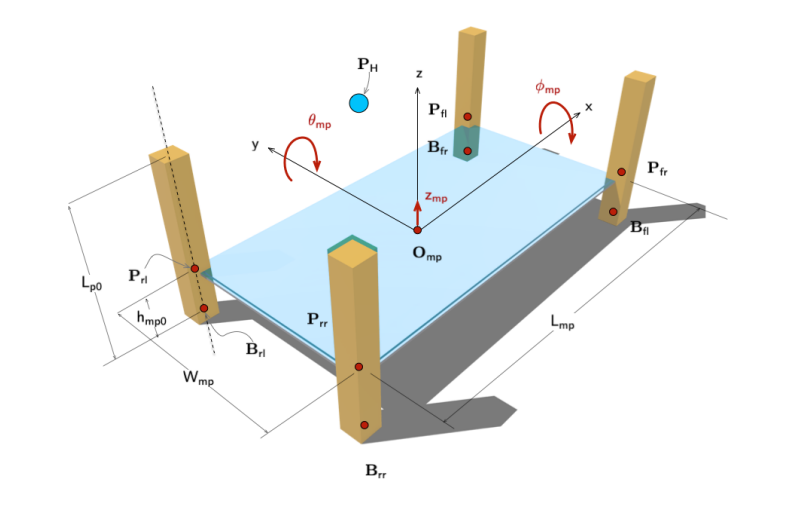
\includegraphics[width=\textwidth]{image_0}
\end{figure}

\newpage
\matlabtitle{Kinematic Analysis}
\begin{par}
\begin{flushleft}
The kinematic and dynamic analysis of the multibody system was performed using the following  linear graph and a global approach.
\end{flushleft}
\end{par}

\begin{par}
\begin{flushleft}
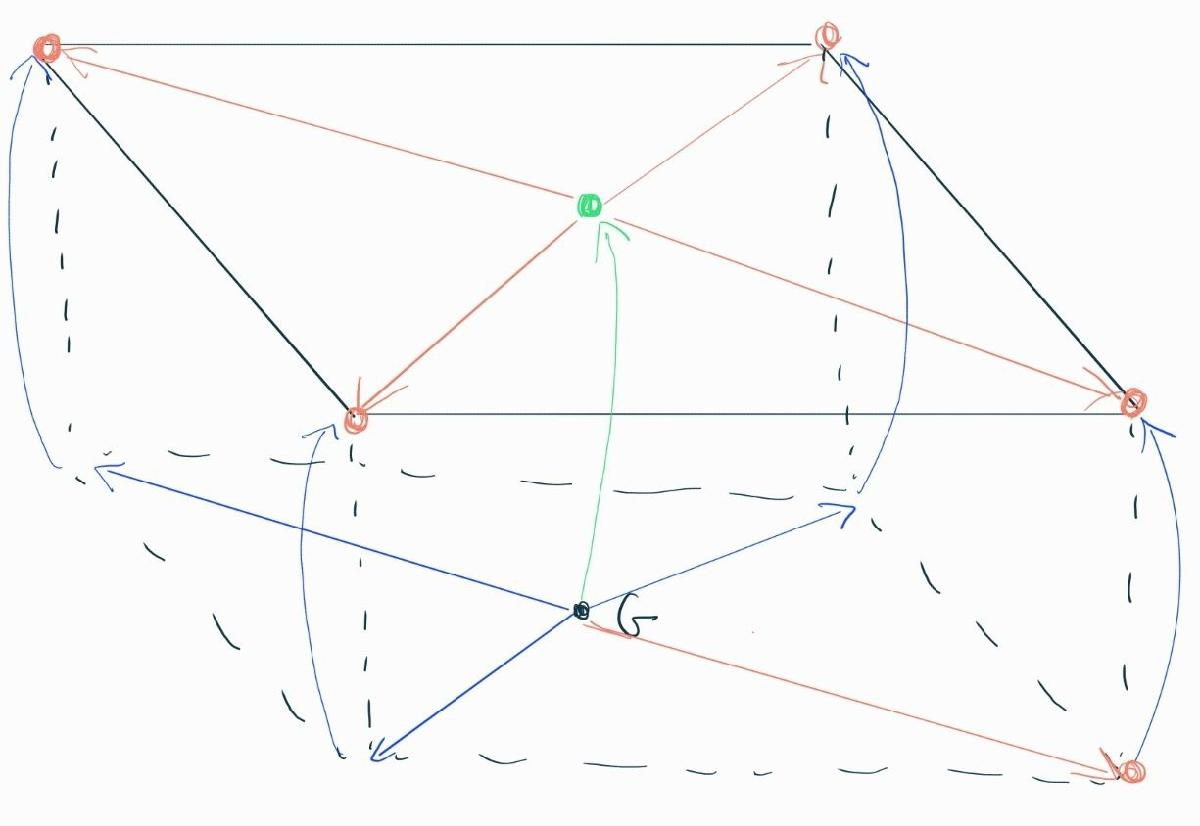
\includegraphics[width=\maxwidth{66.53286502759659em}]{image_1}
\end{flushleft}
\end{par}

\begin{par}
\begin{flushleft}
To solve the kinematic problem, one of the platform's feet is considered fixed, while the other three are treated as joints free to move in the $x$-$y$ plane.
\end{flushleft}
\end{par}

\begin{matlaboutput}
fixed foot translation matrix:
\end{matlaboutput}
\begin{matlaboutput}
    1.0000         0         0   -0.8000
         0    1.0000         0   -0.4100
         0         0    1.0000         0
         0         0         0    1.0000
\end{matlaboutput}
\begin{matlaboutput}
Translation Matrix for a Moving Foot:
\end{matlaboutput}
\begin{matlabsymbolicoutput}
\hskip1em $\displaystyle \left(\begin{array}{cccc}
1 & 0 & 0 & x_{\textrm{rl}} \\
0 & 1 & 0 & y_{\textrm{rl}} \\
0 & 0 & 1 & 0\\
0 & 0 & 0 & 1
\end{array}\right)$
\end{matlabsymbolicoutput}
\begin{par}
\begin{flushleft}
A roto-translation matrix is defined to describe the transformation from the ground to the center of mass of the platform, where rotations occur only around the $x$ and $y$ axes.
\end{flushleft}
\end{par}

\begin{matlabsymbolicoutput}
\hskip1em $\displaystyle \left(\begin{array}{cccc}
\cos \left(\theta_{\textrm{mp}} \right) & 0 & \sin \left(\theta_{\textrm{mp}} \right) & x_{\textrm{mp}} \\
\sin \left(\phi_{\textrm{mp}} \right)\,\sin \left(\theta_{\textrm{mp}} \right) & \cos \left(\phi_{\textrm{mp}} \right) & -\cos \left(\theta_{\textrm{mp}} \right)\,\sin \left(\phi_{\textrm{mp}} \right) & y_{\textrm{mp}} \\
-\cos \left(\phi_{\textrm{mp}} \right)\,\sin \left(\theta_{\textrm{mp}} \right) & \sin \left(\phi_{\textrm{mp}} \right) & \cos \left(\phi_{\textrm{mp}} \right)\,\cos \left(\theta_{\textrm{mp}} \right) & z_{\textrm{mp}} \\
0 & 0 & 0 & 1
\end{array}\right)$
\end{matlabsymbolicoutput}
\begin{par}
\begin{flushleft}
Under the assumption of  small angles, this matrix can be simplified.
\end{flushleft}
\end{par}

\begin{matlabsymbolicoutput}
\hskip1em $\displaystyle \left(\begin{array}{cccc}
1 & 0 & \theta_{\textrm{mp}}  & x_{\textrm{mp}} \\
\phi_{\textrm{mp}} \,\theta_{\textrm{mp}}  & 1 & -\phi_{\textrm{mp}}  & y_{\textrm{mp}} \\
-\theta_{\textrm{mp}}  & \phi_{\textrm{mp}}  & 1 & z_{\textrm{mp}} \\
0 & 0 & 0 & 1
\end{array}\right)$
\end{matlabsymbolicoutput}
\begin{par}
\begin{flushleft}
Fixed transformation matrices are also defined from the platform's center of mass to its edges in local coordinates.
\end{flushleft}
\end{par}

\begin{par}
\begin{flushleft}
The transformations from the base to the top of the actuator are modeled as a prismatic joint, which move vertically on an axis that shares the same rotation as the platform.
\end{flushleft}
\end{par}

\begin{matlabsymbolicoutput}
\hskip1em $\displaystyle \left(\begin{array}{cccc}
\cos \left(\theta_{\textrm{mp}} \right) & 0 & \sin \left(\theta_{\textrm{mp}} \right) & {\textrm{hmp}}_{\textrm{fr}} \,\sin \left(\theta_{\textrm{mp}} \right)\\
\sin \left(\phi_{\textrm{mp}} \right)\,\sin \left(\theta_{\textrm{mp}} \right) & \cos \left(\phi_{\textrm{mp}} \right) & -\cos \left(\theta_{\textrm{mp}} \right)\,\sin \left(\phi_{\textrm{mp}} \right) & -{\textrm{hmp}}_{\textrm{fr}} \,\cos \left(\theta_{\textrm{mp}} \right)\,\sin \left(\phi_{\textrm{mp}} \right)\\
-\cos \left(\phi_{\textrm{mp}} \right)\,\sin \left(\theta_{\textrm{mp}} \right) & \sin \left(\phi_{\textrm{mp}} \right) & \cos \left(\phi_{\textrm{mp}} \right)\,\cos \left(\theta_{\textrm{mp}} \right) & {\textrm{hmp}}_{\textrm{fr}} \,\cos \left(\phi_{\textrm{mp}} \right)\,\cos \left(\theta_{\textrm{mp}} \right)\\
0 & 0 & 0 & 1
\end{array}\right)$
\end{matlabsymbolicoutput}
\begin{par}
\begin{flushleft}
These matrices are then simplified, again under the assumption of small angles.
\end{flushleft}
\end{par}

\begin{matlabsymbolicoutput}
\hskip1em $\displaystyle \left(\begin{array}{cccc}
1 & 0 & \theta_{\textrm{mp}}  & {\textrm{hmp}}_{\textrm{fr}} \,\theta_{\textrm{mp}} \\
\phi_{\textrm{mp}} \,\theta_{\textrm{mp}}  & 1 & -\phi_{\textrm{mp}}  & -{\textrm{hmp}}_{\textrm{fr}} \,\phi_{\textrm{mp}} \\
-\theta_{\textrm{mp}}  & \phi_{\textrm{mp}}  & 1 & {\textrm{hmp}}_{\textrm{fr}} \\
0 & 0 & 0 & 1
\end{array}\right)$
\end{matlabsymbolicoutput}
\begin{par}
\begin{flushleft}
\textbf{Direct kynematics}
\end{flushleft}
\end{par}

\begin{par}
\begin{flushleft}
Equations are created to find the coordinates for the feet, the platform, and a single actuator's length, all based on the lengths of the three other actuators. This is accomplished using the T-graph. It's worth noting that the R-graph equations do not need to be solved, as they are inherently satisfied because the joints undergo the same rotations as the plane itself.
\end{flushleft}
\end{par}

\begin{matlaboutput}
T-graph equations:
\end{matlaboutput}
\begin{matlabsymbolicoutput}
\hskip1em $\displaystyle \begin{array}{l}
\left(\begin{array}{c}
{\textrm{hmp}}_{\textrm{rr}} \,\theta_{\textrm{mp}} -x_{\textrm{mp}} =0\\
\sigma_1 -{\textrm{hmp}}_{\textrm{rr}} \,\phi_{\textrm{mp}} -y_{\textrm{mp}} =0\\
{\textrm{hmp}}_{\textrm{rr}} +\frac{41\,\phi_{\textrm{mp}} }{100}-\frac{4\,\theta_{\textrm{mp}} }{5}-z_{\textrm{mp}} =0\\
x_{\textrm{fl}} -x_{\textrm{mp}} +{\textrm{hmp}}_{\textrm{fl}} \,\theta_{\textrm{mp}} -\frac{4}{5}=0\\
y_{\textrm{fl}} -y_{\textrm{mp}} -{\textrm{hmp}}_{\textrm{fl}} \,\phi_{\textrm{mp}} -\sigma_1 -\frac{41}{100}=0\\
{\textrm{hmp}}_{\textrm{fl}} -\frac{41\,\phi_{\textrm{mp}} }{100}+\frac{4\,\theta_{\textrm{mp}} }{5}-z_{\textrm{mp}} =0\\
x_{\textrm{fr}} -x_{\textrm{mp}} +{\textrm{hmp}}_{\textrm{fr}} \,\theta_{\textrm{mp}} -\frac{4}{5}=0\\
y_{\textrm{fr}} -y_{\textrm{mp}} -{\textrm{hmp}}_{\textrm{fr}} \,\phi_{\textrm{mp}} -\sigma_1 +\frac{41}{100}=0\\
{\textrm{hmp}}_{\textrm{fr}} +\frac{41\,\phi_{\textrm{mp}} }{100}+\frac{4\,\theta_{\textrm{mp}} }{5}-z_{\textrm{mp}} =0\\
x_{\textrm{rl}} -x_{\textrm{mp}} +{\textrm{hmp}}_{\textrm{rl}} \,\theta_{\textrm{mp}} +\frac{4}{5}=0\\
y_{\textrm{rl}} -y_{\textrm{mp}} -{\textrm{hmp}}_{\textrm{rl}} \,\phi_{\textrm{mp}} +\sigma_1 -\frac{41}{100}=0\\
{\textrm{hmp}}_{\textrm{rl}} -\frac{41\,\phi_{\textrm{mp}} }{100}-\frac{4\,\theta_{\textrm{mp}} }{5}-z_{\textrm{mp}} =0
\end{array}\right)\\
\mathrm{}\\
\textrm{where}\\
\mathrm{}\\
\;\;\sigma_1 =\frac{4\,\phi_{\textrm{mp}} \,\theta_{\textrm{mp}} }{5}
\end{array}$
\end{matlabsymbolicoutput}
\begin{matlaboutput}
Direct kynematics solution:
\end{matlaboutput}
\begin{matlaboutput}
hmp_rr: hmp_fr - hmp_fl + hmp_rl
x_mp: (5*hmp_fl^2)/8 - (5*hmp_fl*hmp_rl)/4 - (5*hmp_fr*hmp_fl)/8 +
 	(5*hmp_rl^2)/8 + (5*hmp_fr*hmp_rl)/8
y_mp: (25*hmp_fl^2)/41 - (75*hmp_fl*hmp_fr)/41 - (25*hmp_rl*hmp_fl)/41 + (50*hmp_fr^2)/41 + 
	(25*hmp_rl*hmp_fr)/41
z_mp: hmp_fr/2 + hmp_rl/2
phi_mp: (50*hmp_fl)/41 - (50*hmp_fr)/41
theta_mp: (5*hmp_rl)/8 - (5*hmp_fl)/8
x_fr: (5*hmp_fl^2)/8 - (5*hmp_fl*hmp_rl)/4 + (5*hmp_rl^2)/8 + 4/5
y_fr: -41/100
x_fl: (5*hmp_fl^2)/4 - (15*hmp_fl*hmp_rl)/8 - (5*hmp_fr*hmp_fl)/8 + (5*hmp_rl^2)/8 + 
	(5*hmp_fr*hmp_rl)/8 + 4/5
y_fl: (50*hmp_fl^2)/41 - (100*hmp_fl*hmp_fr)/41 + (50*hmp_fr^2)/41 + 41/100
x_rl: (5*hmp_fr*hmp_rl)/8 - (5*hmp_fl*hmp_rl)/8 - (5*hmp_fl*hmp_fr)/8 + (5*hmp_fl^2)/8 - 4/5
y_rl: (50*hmp_fl^2)/41 - (100*hmp_fl*hmp_fr)/41 + (50*hmp_fr^2)/41 + 41/100
\end{matlaboutput}
\begin{par}
\begin{flushleft}
Next, the results are plotted for three specified actuator heights:
\end{flushleft}
\end{par}

\begin{matlaboutput}
	hrr = 0.19;
	hrl = 0.189;
	hfl = 0.1896;
\end{matlaboutput}

\begin{center}
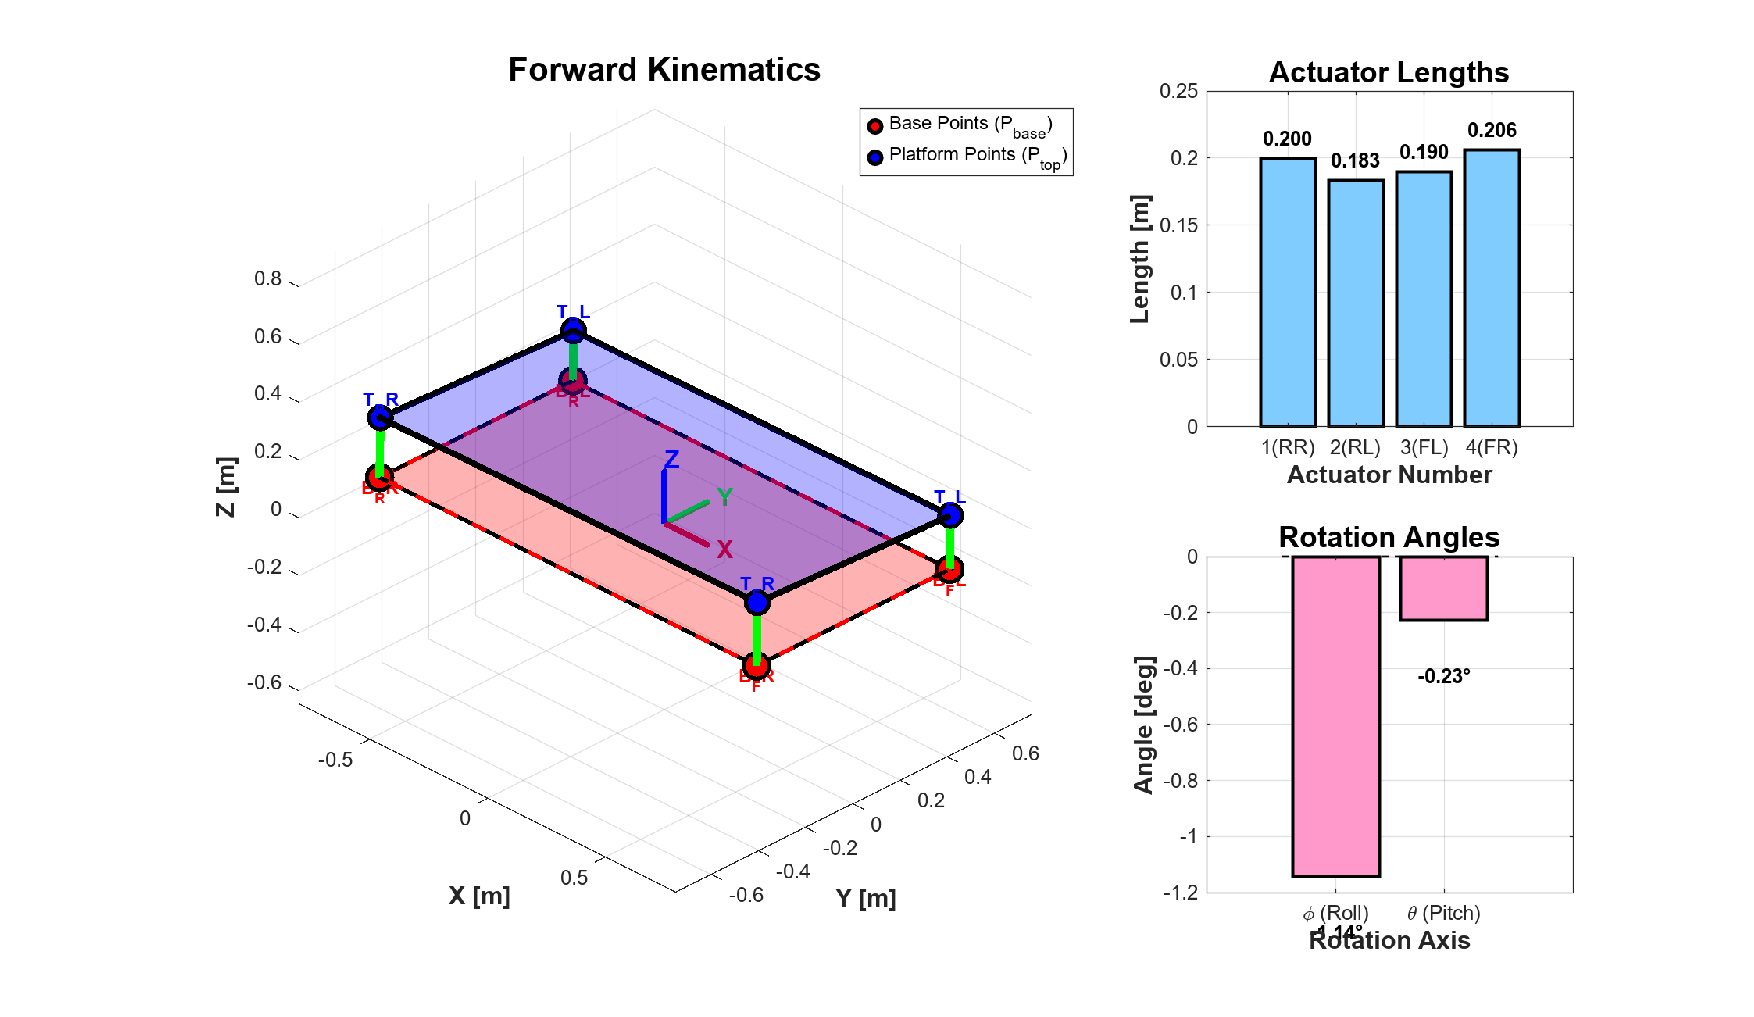
\includegraphics[width=\maxwidth{150cm}]{figure_0.eps}
\end{center}
\begin{par}
\begin{flushleft}
\textbf{Inverse kynematics}
\end{flushleft}
\end{par}

\begin{par}
\begin{flushleft}
The inverse kinematics can be derived from the same set of equations obtained from the T-Graph. This allows the required actuator lengths to be computed for a given platform pose (position and orientation).
\end{flushleft}
\end{par}

\begin{matlaboutput}
    hmp_fr: z_mp - (4*theta_mp)/5 - (41*phi_mp)/100
    hmp_rr: (4*theta_mp)/5 - (41*phi_mp)/100 + z_mp
    hmp_rl: (41*phi_mp)/100 + (4*theta_mp)/5 + z_mp
    hmp_fl: (41*phi_mp)/100 - (4*theta_mp)/5 + z_mp
      x_mp: (theta_mp*(80*theta_mp - 41*phi_mp + 100*z_mp))/100
      y_mp: (41*phi_mp^2)/100 - z_mp*phi_mp
      x_fr: (8*theta_mp^2)/5 + 4/5
      y_fr: -41/100
      x_fl: (8*theta_mp^2)/5 - (41*phi_mp*theta_mp)/50 + 4/5
      y_fl: (41*phi_mp^2)/50 + 41/100
      x_rl: - (41*phi_mp*theta_mp)/50 - 4/5
      y_rl: (41*phi_mp^2)/50 + 41/100
\end{matlaboutput}
\begin{par}
\begin{flushleft}
To verify the self-consistency of the models, the $z$, $\phi$, and $\theta$ values obtained from the direct dynamics simulation were used as inputs for the inverse dynamics model. This test confirmed that the resulting system configuration is identical to the original one, thus validating the approach
\end{flushleft}
\end{par}


\begin{center}
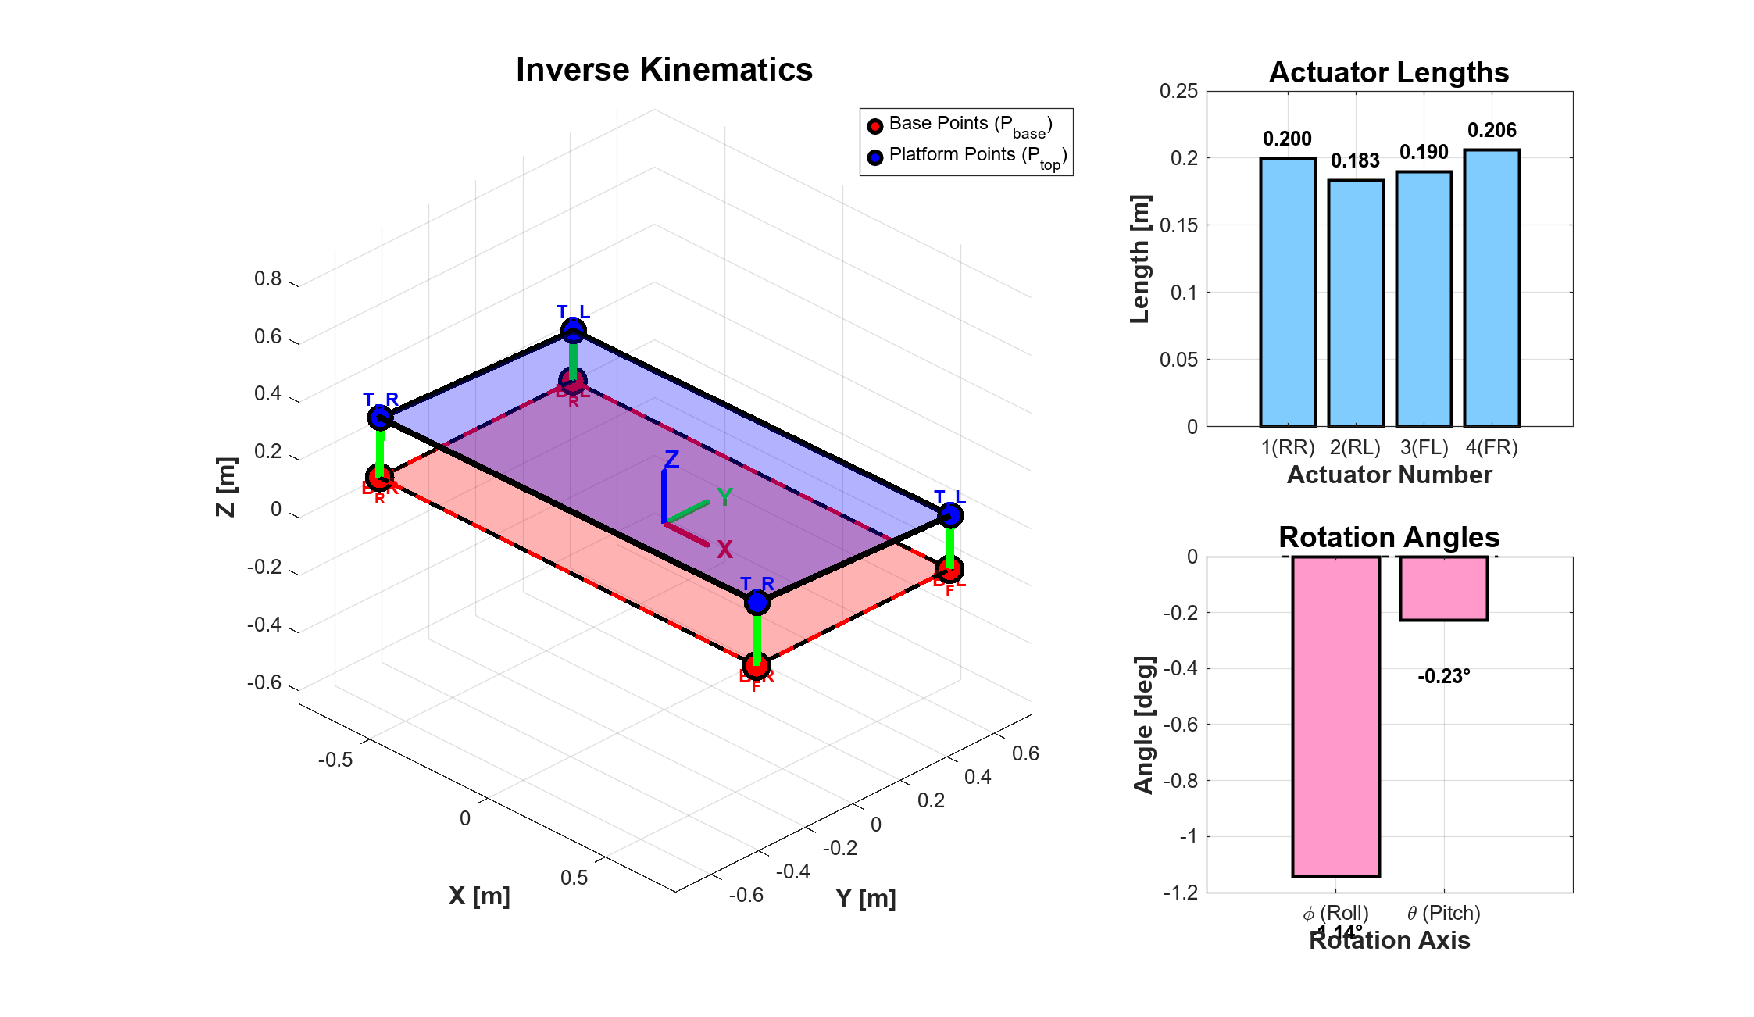
\includegraphics[width=\maxwidth{127.84746613146011em}]{figure_1.eps}
\end{center}
\begin{par}
\begin{flushleft}
\textbf{Motion ranges}
\end{flushleft}
\end{par}

\begin{par}
\begin{flushleft}
The system's workspace is evaluated based on the assumption that each actuator can travel $\pm50\%$ of its full stroke from a central position.
\end{flushleft}
\end{par}

\begin{par}
\begin{flushleft}
The motion ranges are determined by evaluating the system's behavior at maximum and minimum actuator lengths. For small angles, the equations for each actuator's length are linear and independent. Therefore, the principle of superposition is applied: the system's total displacement is calculated as the sum of individual behaviors. This is done by varying one degree of freedom at a time while keeping the other two constant to isolate their effects.
\end{flushleft}
\end{par}

\begin{figure}[H]
	\centering
	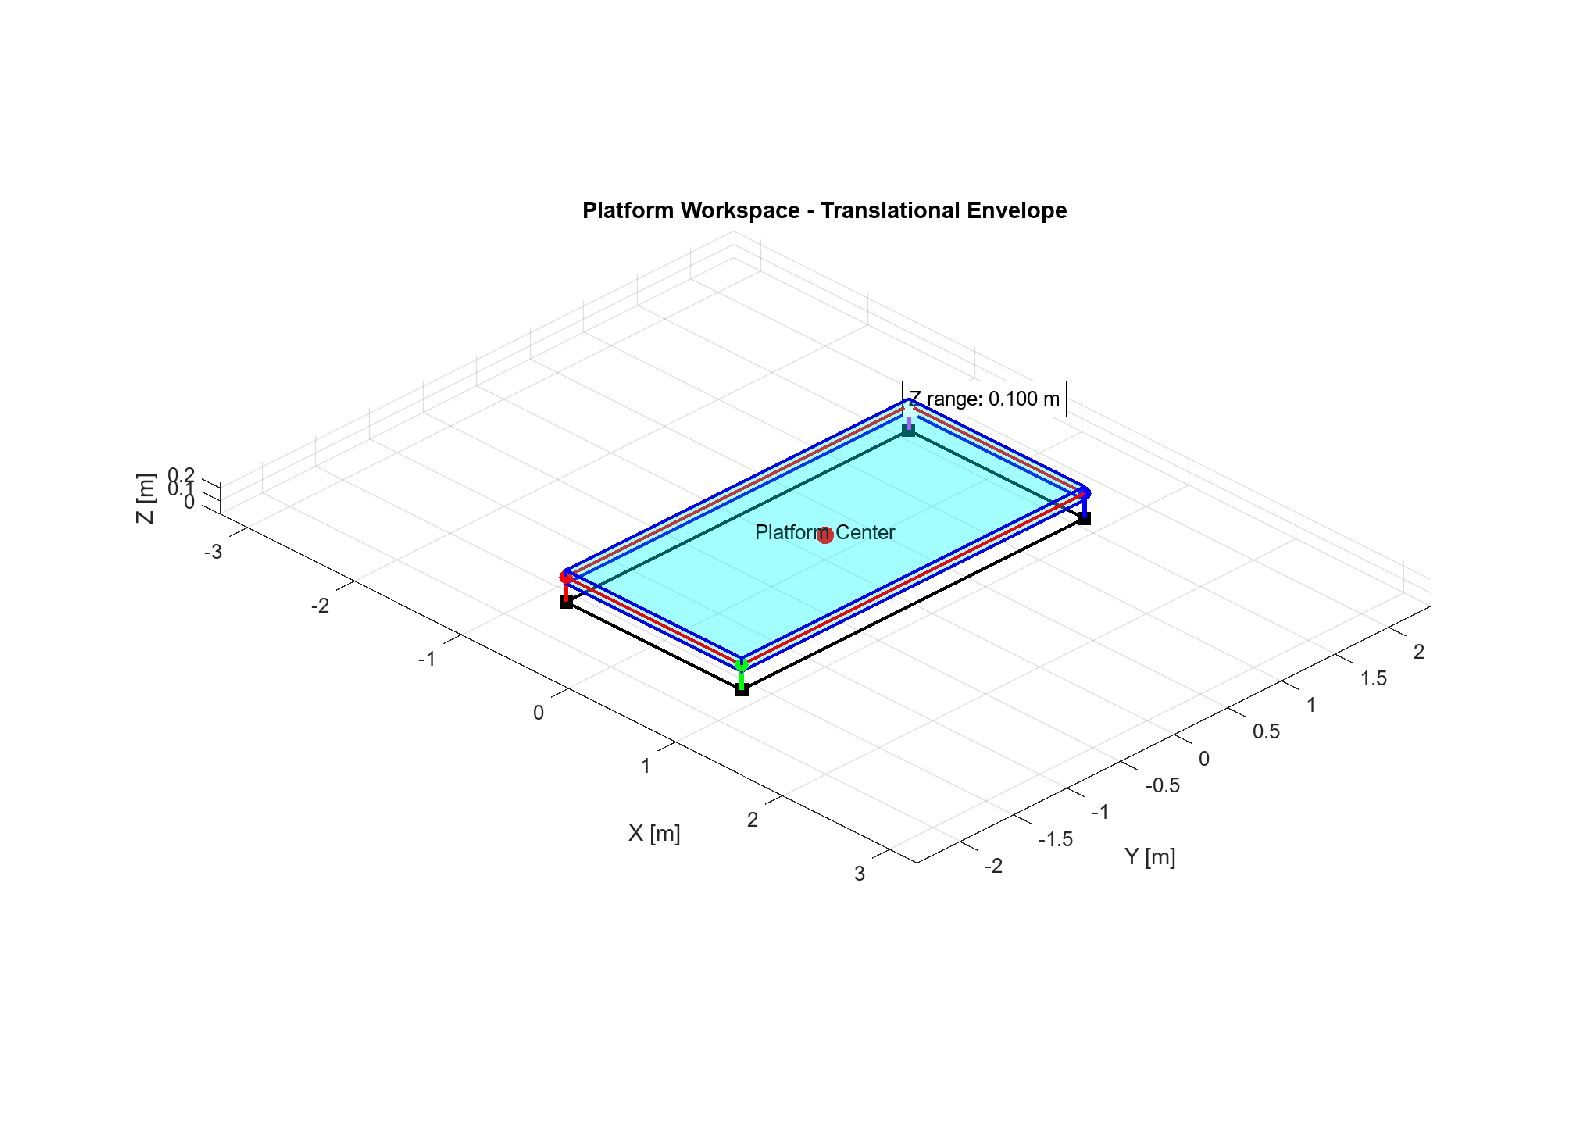
\includegraphics[width=0.9\textwidth]{figure_2.eps}
	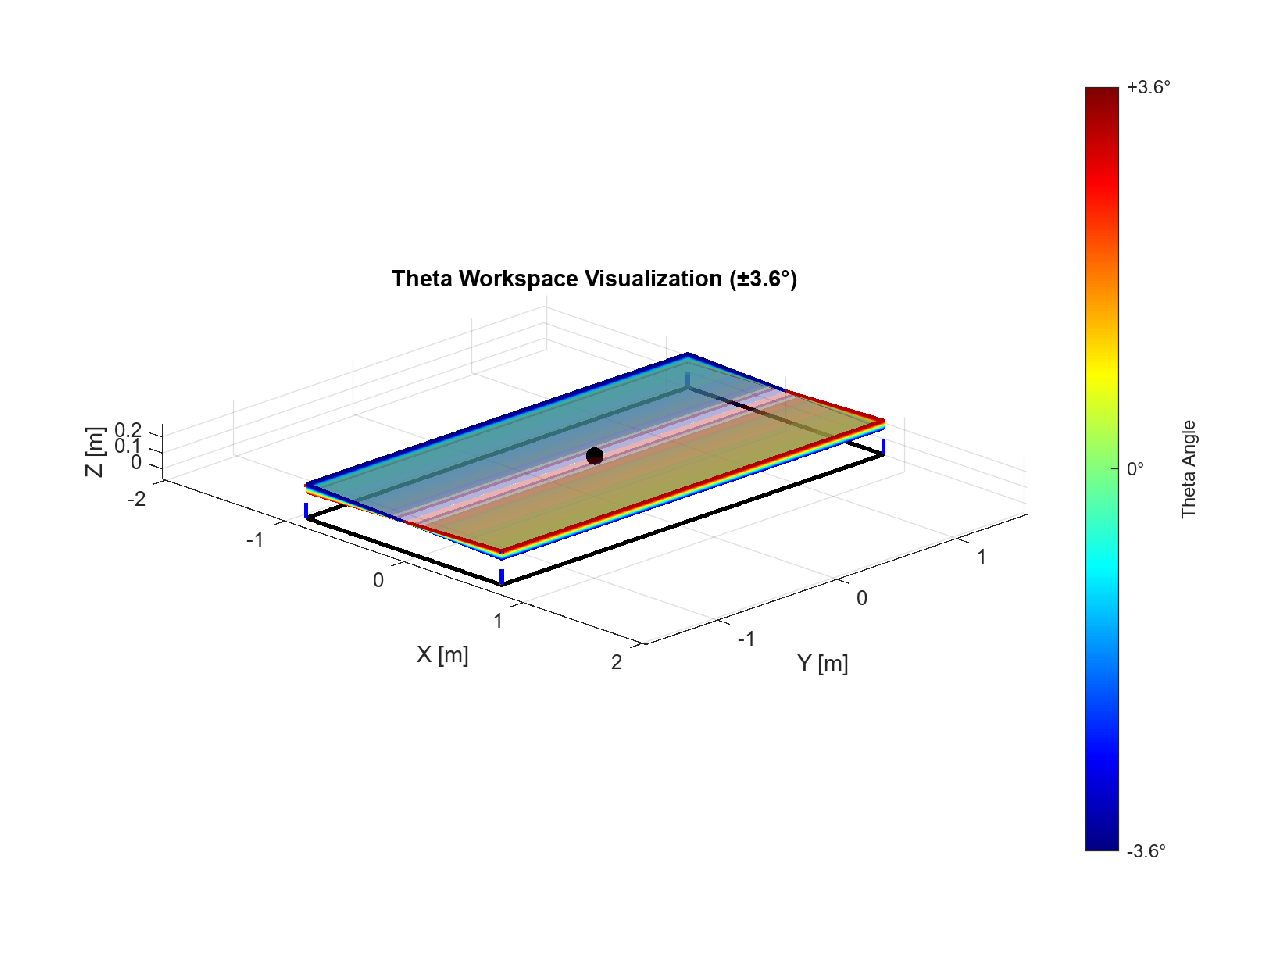
\includegraphics[width=0.9\textwidth]{figure_3.eps}
\end{figure}

\begin{figure}[H]
	\centering
	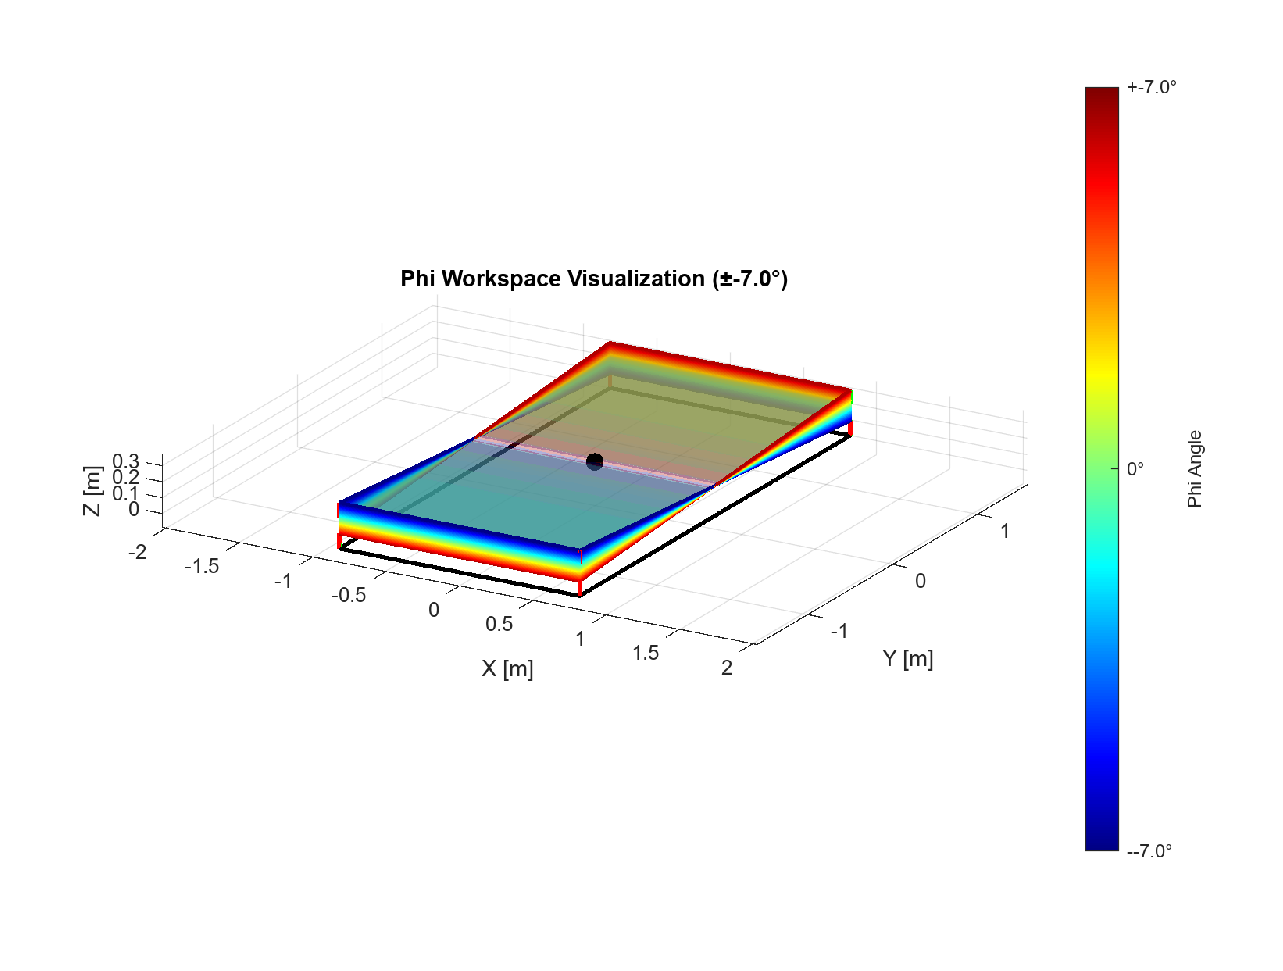
\includegraphics[width=0.9\textwidth]{figure_4.eps}
	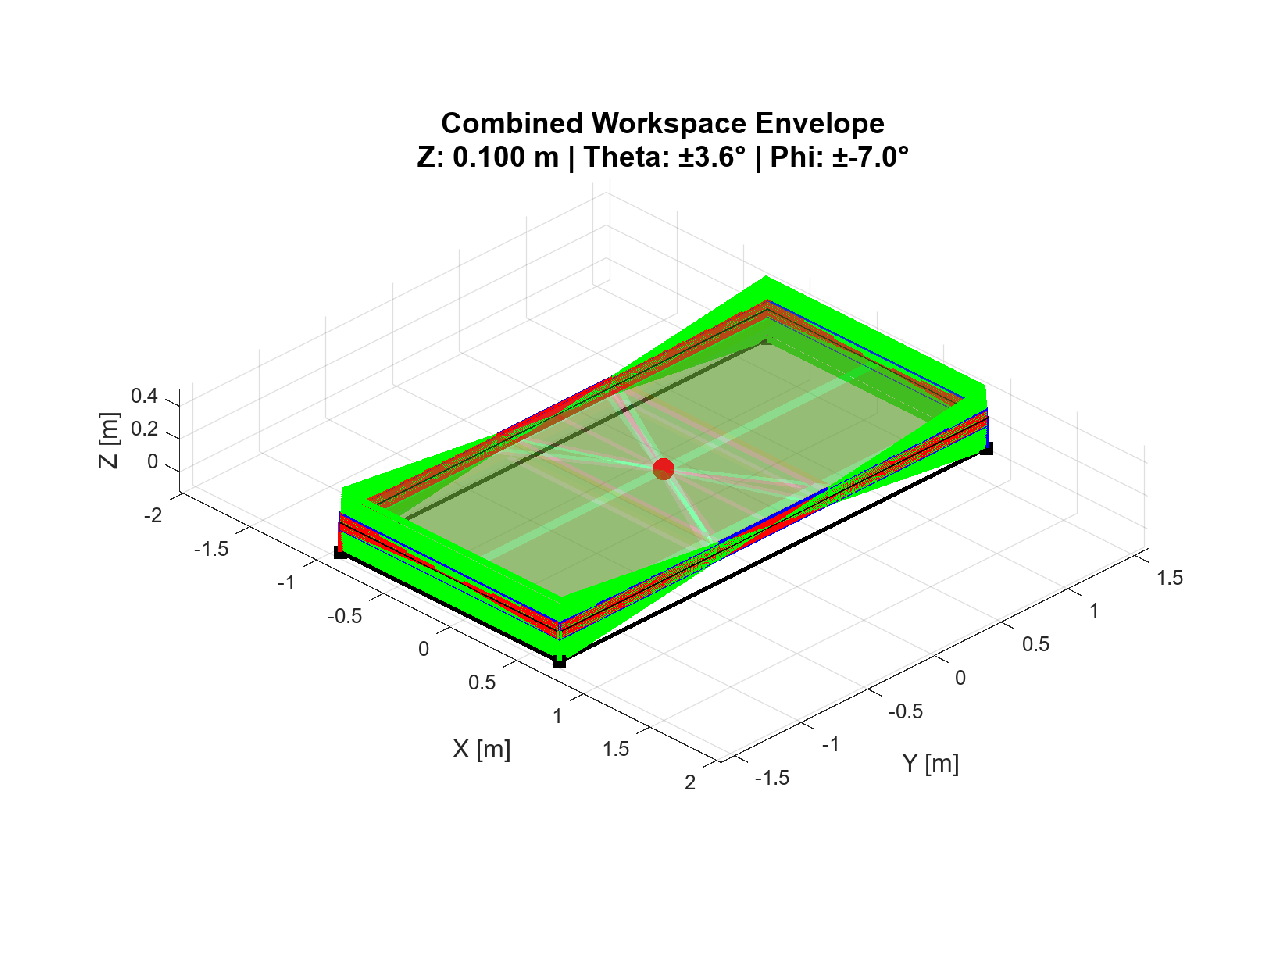
\includegraphics[width=0.9\textwidth]{figure_5.eps}
\end{figure}


\begin{par}
\begin{flushleft}
The resulting theoretical motion ranges are summarized as follows:
\end{flushleft}
\end{par}

\begin{itemize}
\setlength{\itemsep}{-1ex}
   \item{\begin{flushleft} $z$ (heave): $\pm50 mm$ \end{flushleft}}
   \item{\begin{flushleft} $\Theta$ (pitch): $\pm3.581$ degrees \end{flushleft}}
   \item{\begin{flushleft} $\Phi$ (roll): $\pm6.9873$ degrees \end{flushleft}}
\end{itemize}

\begin{par}
\begin{flushleft}
This confirms that the small-angle assumptions are valid. The following ranges represent the maximum and minimum for each degree of freedom when the others are inactive. Naturally, if other degrees of freedom have non-zero values, the available range for any given degree of freedom will be more restricted.
\end{flushleft}
\end{par}

\begin{par}
\begin{flushleft}
A discrepancy was noted between the calculated ranges for pitch and roll and those specified in the datasheet. This difference is resolved by repeating the calculation using the plate dimensions from the datasheet, which are slightly smaller than those provided in the assignment. Using the datasheet dimensions yields results that perfectly match the specified ranges for both angles.
\end{flushleft}
\end{par}

\begin{par}
\begin{flushleft}
\textbf{Pilot}
\end{flushleft}
\end{par}

\begin{par}
\begin{flushleft}
To compute the velocity and acceleration perceived by the driver, a point is defined to represent the position of their head. The driver is modeled as a rigid body (xp,yp,zp), whose movement is not autonomous but rather an indirect effect of the motion of the plate on which it rests. The resulting velocity and acceleration are then calculated at that specific point within the body-fixed frame.
\end{flushleft}
\end{par}

\begin{matlaboutput}
pilot position:
\end{matlaboutput}
\begin{matlabsymbolicoutput}
\hskip1em $\displaystyle \left(\begin{array}{c}
\textrm{xp}+x_{\textrm{mp}} \left(t\right)+\textrm{zp}\,\theta_{\textrm{mp}} \left(t\right)\\
\textrm{yp}+y_{\textrm{mp}} \left(t\right)-\textrm{zp}\,\phi_{\textrm{mp}} \left(t\right)+\textrm{xp}\,\phi_{\textrm{mp}} \left(t\right)\,\theta_{\textrm{mp}} \left(t\right)\\
\textrm{zp}+z_{\textrm{mp}} \left(t\right)+\textrm{yp}\,\phi_{\textrm{mp}} \left(t\right)-\textrm{xp}\,\theta_{\textrm{mp}} \left(t\right)
\end{array}\right)$
\end{matlabsymbolicoutput}
\begin{matlaboutput}
pilot linear velocity
\end{matlaboutput}
\begin{matlabsymbolicoutput}
\hskip1em $\displaystyle \left(\begin{array}{c}
\textrm{zp}\,\frac{\partial }{\partial t}\;\theta_{\textrm{mp}} \left(t\right)+\frac{\partial }{\partial t}\;x_{\textrm{mp}} \left(t\right)\\
\frac{\partial }{\partial t}\;y_{\textrm{mp}} \left(t\right)-\textrm{zp}\,\frac{\partial }{\partial t}\;\phi_{\textrm{mp}} \left(t\right)+\textrm{xp}\,\phi_{\textrm{mp}} \left(t\right)\,\frac{\partial }{\partial t}\;\theta_{\textrm{mp}} \left(t\right)+\textrm{xp}\,\theta_{\textrm{mp}} \left(t\right)\,\frac{\partial }{\partial t}\;\phi_{\textrm{mp}} \left(t\right)\\
\textrm{yp}\,\frac{\partial }{\partial t}\;\phi_{\textrm{mp}} \left(t\right)-\textrm{xp}\,\frac{\partial }{\partial t}\;\theta_{\textrm{mp}} \left(t\right)+\frac{\partial }{\partial t}\;z_{\textrm{mp}} \left(t\right)
\end{array}\right)$
\end{matlabsymbolicoutput}
\begin{matlaboutput}
pilot linear accelleration
\end{matlaboutput}
\begin{matlabsymbolicoutput}
\hskip1em $\displaystyle \begin{array}{l}
\left(\begin{array}{c}
\textrm{zp}\,\sigma_1 +\frac{\partial^2 }{\partial t^2 }\;x_{\textrm{mp}} \left(t\right)\\
\frac{\partial^2 }{\partial t^2 }\;y_{\textrm{mp}} \left(t\right)-\textrm{zp}\,\sigma_2 +2\,\textrm{xp}\,\frac{\partial }{\partial t}\;\theta_{\textrm{mp}} \left(t\right)\,\frac{\partial }{\partial t}\;\phi_{\textrm{mp}} \left(t\right)+\textrm{xp}\,\phi_{\textrm{mp}} \left(t\right)\,\sigma_1 +\textrm{xp}\,\theta_{\textrm{mp}} \left(t\right)\,\sigma_2 \\
\textrm{yp}\,\sigma_2 -\textrm{xp}\,\sigma_1 +\frac{\partial^2 }{\partial t^2 }\;z_{\textrm{mp}} \left(t\right)-\frac{981}{100}
\end{array}\right)\\
\mathrm{}\\
\textrm{where}\\
\mathrm{}\\
\;\;\sigma_1 =\frac{\partial^2 }{\partial t^2 }\;\theta_{\textrm{mp}} \left(t\right)\\
\mathrm{}\\
\;\;\sigma_2 =\frac{\partial^2 }{\partial t^2 }\;\phi_{\textrm{mp}} \left(t\right)
\end{array}$
\end{matlabsymbolicoutput}
\begin{matlaboutput}
pilot angular velocity
\end{matlaboutput}
\begin{matlabsymbolicoutput}
\hskip1em $\displaystyle \left(\begin{array}{c}
\frac{\partial }{\partial t}\;\phi_{\textrm{mp}} \left(t\right)\\
\frac{\partial }{\partial t}\;\theta_{\textrm{mp}} \left(t\right)-\phi_{\textrm{mp}} \left(t\right)\,\theta_{\textrm{mp}} \left(t\right)\,\frac{\partial }{\partial t}\;\phi_{\textrm{mp}} \left(t\right)\\
\theta_{\textrm{mp}} \left(t\right)\,\frac{\partial }{\partial t}\;\phi_{\textrm{mp}} \left(t\right)
\end{array}\right)$
\end{matlabsymbolicoutput}
\begin{matlaboutput}
pilot angular accelleration
\end{matlaboutput}
\begin{matlabsymbolicoutput}
\hskip1em $\displaystyle \begin{array}{l}
\left(\begin{array}{c}
{\theta_{\textrm{mp}} \left(t\right)}^2 \,\sigma_1 +\sigma_1 +2\,\theta_{\textrm{mp}} \left(t\right)\,\frac{\partial }{\partial t}\;\theta_{\textrm{mp}} \left(t\right)\,\frac{\partial }{\partial t}\;\phi_{\textrm{mp}} \left(t\right)\\
\sigma_3 -\theta_{\textrm{mp}} \left(t\right)\,\sigma_2 -\phi_{\textrm{mp}} \left(t\right)\,\theta_{\textrm{mp}} \left(t\right)\,\sigma_1 -\phi_{\textrm{mp}} \left(t\right)\,\frac{\partial }{\partial t}\;\theta_{\textrm{mp}} \left(t\right)\,\frac{\partial }{\partial t}\;\phi_{\textrm{mp}} \left(t\right)\\
-\theta_{\textrm{mp}} \left(t\right)\,{\phi_{\textrm{mp}} \left(t\right)}^2 \,\sigma_1 +\phi_{\textrm{mp}} \left(t\right)\,\sigma_3 -2\,\theta_{\textrm{mp}} \left(t\right)\,\phi_{\textrm{mp}} \left(t\right)\,\sigma_2 -\frac{\partial }{\partial t}\;\theta_{\textrm{mp}} \left(t\right)\,{\phi_{\textrm{mp}} \left(t\right)}^2 \,\frac{\partial }{\partial t}\;\phi_{\textrm{mp}} \left(t\right)+\frac{\partial }{\partial t}\;\theta_{\textrm{mp}} \left(t\right)\,\frac{\partial }{\partial t}\;\phi_{\textrm{mp}} \left(t\right)
\end{array}\right)\\
\mathrm{}\\
\textrm{where}\\
\mathrm{}\\
\;\;\sigma_1 =\frac{\partial^2 }{\partial t^2 }\;\phi_{\textrm{mp}} \left(t\right)\\
\mathrm{}\\
\;\;\sigma_2 ={{\left(\frac{\partial }{\partial t}\;\phi_{\textrm{mp}} \left(t\right)\right)}}^2 \\
\mathrm{}\\
\;\;\sigma_3 =\frac{\partial^2 }{\partial t^2 }\;\theta_{\textrm{mp}} \left(t\right)
\end{array}$
\end{matlabsymbolicoutput}
\newpage
\matlabtitle{Dynamic Modeling}

\begin{par}
\begin{flushleft}
To ensure efficient computation time for the dynamic analysis, a reduction in the number of coordinates and constraints is necessary. The methodology is as follows:
\end{flushleft}
\end{par}

\begin{enumerate}
\setlength{\itemsep}{-1ex}
   \item{\begin{flushleft} Selection of Coordinates: A set of generalized coordinates, q, is chosen to include the platform's vertical position ($z_mp$), its pitch ($\theta_mp$) and roll ($\phi_mp$) angles, and the four actuator heights ($hmp$). \end{flushleft}}
   \item{\begin{flushleft} Imposing Constraints: The relevant constraint for the generalized coordinates are selected from the T-graph equations. The motion of three actuators is defined as a prescribed function of time. This allows their lengths to be treated as direct inputs for the system analysis. \end{flushleft}}
   \item{\begin{flushleft} Resulting System: By defining the motion of three actuators, the platform's three degrees of freedom are effectively constrained, reducing the system's final degrees of freedom to zero. \end{flushleft}}
\end{enumerate}


\begin{matlaboutput}
Constraints equations:
\end{matlaboutput}
\begin{matlabsymbolicoutput}
\hskip1em $\displaystyle \begin{array}{l}
\left(\begin{array}{c}
{\textrm{hmp}}_{\textrm{rr}} \left(t\right)+\sigma_2 -\sigma_1 -z_{\textrm{mp}} \left(t\right)=0\\
{\textrm{hmp}}_{\textrm{fl}} \left(t\right)-\sigma_2 +\sigma_1 -z_{\textrm{mp}} \left(t\right)=0\\
{\textrm{hmp}}_{\textrm{fr}} \left(t\right)+\sigma_2 +\sigma_1 -z_{\textrm{mp}} \left(t\right)=0\\
{\textrm{hmp}}_{\textrm{rl}} \left(t\right)-\sigma_2 -\sigma_1 -z_{\textrm{mp}} \left(t\right)=0\\
{\textrm{hmp}}_{\textrm{fr}} \left(t\right)-f_1 \left(t\right)=0\\
{\textrm{hmp}}_{\textrm{rl}} \left(t\right)-f_2 \left(t\right)=0\\
{\textrm{hmp}}_{\textrm{fl}} \left(t\right)-f_3 \left(t\right)=0
\end{array}\right)\\
\mathrm{}\\
\textrm{where}\\
\mathrm{}\\
\;\;\sigma_1 =\frac{4\,\theta_{\textrm{mp}} \left(t\right)}{5}\\
\mathrm{}\\
\;\;\sigma_2 =\frac{41\,\phi_{\textrm{mp}} \left(t\right)}{100}
\end{array}$
\end{matlabsymbolicoutput}

\vspace{1em}
\begin{matlaboutput}
Rank of Jacobian: 7
\end{matlaboutput}
\begin{matlaboutput}
Number of constraints (M): 7
\end{matlaboutput}
\begin{matlaboutput}
Number of generalized coordinates (N): 7
\end{matlaboutput}
\begin{matlaboutput}
The constraints are linearly independent in this configuration.
\end{matlaboutput}
\begin{matlaboutput}
Number of DOF: 0
\end{matlaboutput}
\begin{par}
\begin{flushleft}
As expected, using three additional constraints to control the actuator positions as a function of time has reduced the system's degrees of freedom (DOF) to zero. Otherwise, if the actuators had been controlled by force instead of by adding a constraint, the system would have had three degrees of freedom. 
\end{flushleft}
\end{par}

\begin{par}
\begin{flushleft}
Subsequently, the potential and kinetic energy are expressed as a function of the generalized coordinates in order to use the energy in the Lagrangian formulation:
\end{flushleft}
\end{par}

\begin{par}
                                                                                                                                                                            $$\frac{d}{\textrm{dt}}\left(\frac{\textrm{dL}}{{{\textrm{dq}}_i }^{\prime } }\right)-\frac{\textrm{dL}}{{\textrm{dq}}_i }-\lambda \frac{d\Phi }{{\textrm{dq}}_i }=Q_i$$
\end{par}

\begin{matlaboutput}
kinetic energy:
\end{matlaboutput}
\begin{matlabsymbolicoutput}
\hskip1em $\displaystyle 15\,{{\left(\frac{\partial }{\partial t}\;{\textrm{hmp}}_{\textrm{fl}} \left(t\right)\right)}}^2 +15\,{{\left(\frac{\partial }{\partial t}\;{\textrm{hmp}}_{\textrm{fr}} \left(t\right)\right)}}^2 +15\,{{\left(\frac{\partial }{\partial t}\;{\textrm{hmp}}_{\textrm{rl}} \left(t\right)\right)}}^2 +15\,{{\left(\frac{\partial }{\partial t}\;{\textrm{hmp}}_{\textrm{rr}} \left(t\right)\right)}}^2 +\frac{4156625437653019\,{{\left(\frac{\partial }{\partial t}\;\phi_{\textrm{mp}} \left(t\right)\right)}}^2 }{281474976710656}+\frac{1371470290886227\,{{\left(\frac{\partial }{\partial t}\;\theta_{\textrm{mp}} \left(t\right)\right)}}^2 }{70368744177664}+75\,{{\left(\frac{\partial }{\partial t}\;z_{\textrm{mp}} \left(t\right)\right)}}^2 +\frac{192\,{{\left(\phi_{\textrm{mp}} \left(t\right)\,\frac{\partial }{\partial t}\;\theta_{\textrm{mp}} \left(t\right)+\theta_{\textrm{mp}} \left(t\right)\,\frac{\partial }{\partial t}\;\phi_{\textrm{mp}} \left(t\right)\right)}}^2 }{5}$
\end{matlabsymbolicoutput}
\begin{matlaboutput}
potential energy:
\end{matlaboutput}
\begin{matlabsymbolicoutput}
\hskip1em $\displaystyle \frac{2943\,{\textrm{hmp}}_{\textrm{fl}} \left(t\right)}{10}+\frac{2943\,{\textrm{hmp}}_{\textrm{fr}} \left(t\right)}{10}+\frac{2943\,{\textrm{hmp}}_{\textrm{rl}} \left(t\right)}{10}+\frac{2943\,{\textrm{hmp}}_{\textrm{rr}} \left(t\right)}{10}+\frac{2943\,z_{\textrm{mp}} \left(t\right)}{2}$
\end{matlabsymbolicoutput}
\begin{matlaboutput}
Equations of Motion for the Generalized Variables:
\end{matlaboutput}
\begin{matlaboutput}
sol_d = struct with fields:
    a1: lambda1/150 + lambda2/150 + lambda3/150 + lambda4/150 - 981/100
    a2: -(35184372088832*(281151409631676535*lambda1 - 281151409631676535*lambda2 + …
    a3: -(140737488355328*(103915635941325475*lambda2 - 103915635941325475*lambda1 + …
    a4: - lambda1/30 - 981/100
    a5: - lambda4/30 - lambda6/30 - 981/100
    a6: - lambda2/30 - lambda7/30 - 981/100
    a7: - lambda3/30 - lambda5/30 - 981/100

\end{matlaboutput}
\begin{par}
\begin{flushleft}
The resulting system is a set of Differential-Algebraic Equations (DAE), composed of both a differential part (the equations of motion) and an algebraic part (the constraint equations).
\end{flushleft}
\end{par}

\matlabheadingtwo{Index Reduction and converting the model for numerical solution}

\begin{par}
\begin{flushleft}
To determine the index of the DAE, we compute the Jacobian of the constraint equations with respect to the Lagrange multipliers. If the Jacobian is not full-rank, the constraints cannot yet be solved for the multipliers, indicating an index greater than 1.
\end{flushleft}
\end{par}


\begin{matlaboutput}
max_rank: 7 | Rank: 0 | Determinant is non-zero: false
\end{matlaboutput}
\begin{par}
\begin{flushleft}
As expected, the Jacobian is singular, confirming that the system is not of index-1. We proceed to differentiate the constraint equations once with respect to time, and substitute the known expressions for the derivatives.
\end{flushleft}
\end{par}

\matlabheadingthree{First derivation}

\begin{par}
\begin{flushleft}
These are the velocity-level (first derivative) constraints. However, their Jacobian is still not full-rank:
\end{flushleft}
\end{par}

\begin{matlaboutput}
max_rank: 7 | Rank: 0 | Determinant is non-zero: false
\end{matlaboutput}
\begin{par}
\begin{flushleft}
\textbf{Second derivation}
\end{flushleft}
\end{par}

\begin{matlaboutput}
max_rank: 7 | Rank: 7 | Determinant is non-zero: true
\end{matlaboutput}
\begin{par}
\begin{flushleft}
This time, the Jacobian is full-rank and nonsingular. This confirms that the system has been reduced to index-1, and is now in a form suitable for numerical integration. The system is formally of index-3, as two differentiations were required.
\end{flushleft}
\end{par}

\begin{par}
\begin{flushleft}
Finally, we solve the second-derivative constraint system to obtain explicit expressions for the Lagrange multipliers.
\end{flushleft}
\end{par}

\begin{matlaboutput}
Equation of the lagrange multiplier
\end{matlaboutput}
\begin{matlaboutput}
    lambda1: 30*diff(f_3(t), t, t) - 30*diff(f_2(t), t, t) - 30*diff(f_1(t), t, t) - 2943/10
    lambda2: 30*phi_mp(t)^2*diff(f_3(t), t, t) - 30*phi_mp(t)^2*diff(f_2(t), t, t) - …
    lambda3: (192000*theta_mp(t)^2*diff(f_1(t), t, t))/1681 - …
    lambda4: 30*phi_mp(t)^2*diff(f_2(t), t, t) - 30*phi_mp(t)^2*diff(f_3(t), t, t) + …
    lambda5: (192000*theta_mp(t)^2*diff(f_3(t), t, t))/1681 - (192000*theta_mp(t)^2* …
    lambda6: 30*phi_mp(t)^2*diff(f_3(t), t, t) - 30*phi_mp(t)^2*diff(f_2(t), t, t) - …
    lambda7: 30*phi_mp(t)^2*diff(f_2(t), t, t) - 30*phi_mp(t)^2*diff(f_3(t), t, t) + …
\end{matlaboutput}

\newpage
\matlabtitle{System Response Analysis}


\begin{par}
\begin{flushleft}
Once the system has been reduced to index-1, we can numerically integrate it using a standard ODE solver. In this case, we use ode45. Before doing so, it is essential to ensure that the initial state satisfies both the position-level and velocity-level constraints, otherwise numerical errors will grow rapidly over time.
\end{flushleft}
\end{par}

\begin{par}
\begin{flushleft}
\textbf{Sinusoidal}
\end{flushleft}
\end{par}

\begin{par}
\begin{flushleft}
For the system analysis, three functions $f_1$, $f_2$, and $f_3$ are defined. These functions serve as the time-varying length inputs for the actuators.
\end{flushleft}
\end{par}

\begin{matlabsymbolicoutput}
$f_1$:

\hskip1em $\displaystyle \frac{\sin \left(t\right)}{40}+\frac{3549}{10000}$

$f_2$:

\hskip1em $\displaystyle \frac{\sin \left(\frac{11\,t}{10}\right)}{1000}+\frac{3549}{10000}$

$f_3$:

\hskip1em $\displaystyle \frac{3\,\sin \left(t\right)}{100}+\frac{3549}{10000}$
\end{matlabsymbolicoutput}
\begin{par}
\begin{flushleft}
The solution to the Ordinary Differential Equation (ODE) is initiated by defining the initial conditions, which are derived from the  constraints functions 
\end{flushleft}
\end{par}

\begin{matlaboutput}
Initial state of the generalized coordinates and their first-order derivatives:
\end{matlaboutput}
\begin{matlabsymbolicoutput}
\hskip1em $\displaystyle \left(\begin{array}{cccccccccccccc}
\frac{3549}{10000} & 0 & 0 & \frac{3549}{10000} & \frac{3549}{10000} & \frac{3549}{10000} & \frac{3549}{10000} & \frac{261}{20000} & \frac{1}{164} & -\frac{289}{16000} & -\frac{39}{10000} & \frac{11}{10000} & \frac{3}{100} & \frac{1}{40}
\end{array}\right)$
\end{matlabsymbolicoutput}
\begin{par}
\begin{flushleft}
This check ensures that both the holonomic and hidden (velocity-level) constraints are satisfied at time zero. Failing to meet these would invalidate the results of any integration process.
\end{flushleft}
\end{par}

\matlabheadingthree{Integration}

\begin{par}
\begin{flushleft}
Next, the system of differential equations is defined. This is achieved by substituting the previously solved expressions for the Lagrange multipliers into the DAE, effectively converting the system into a set of Ordinary Differential Equations (ODEs).
\end{flushleft}
\end{par}


\begin{par}
\begin{flushleft}
The results obtained for the sinusoidal inputs are now presented below.
\end{flushleft}
\end{par}


\begin{par}
\begin{flushleft}
\textbf{Impulse}
\end{flushleft}
\end{par}

\begin{par}
\begin{flushleft}
For the system analysis, three functions $f_1$, $f_2$, and $f_3$ are defined. These functions serve as the time-varying length inputs for the actuators.

Since a true impulse cannot be generated numerically, the sigmoid function was chosen as a smooth and stable approximation that avoids numerical errors.
\end{flushleft}
\end{par}

\begin{matlabsymbolicoutput}
$f_1$:

\hskip1em $\displaystyle \frac{17}{200\,{\left({\mathrm{e}}^{5-5\,t} +1\right)}}$

$f_2$:

\hskip1em $\displaystyle \frac{1}{20\,{\left({\mathrm{e}}^{5-5\,t} +1\right)}}$

$f_3$:

\hskip1em $\displaystyle \frac{1243}{20000\,{\left({\mathrm{e}}^{5-5\,t} +1\right)}}$
\end{matlabsymbolicoutput}
\matlabheadingthree{Integration}

\begin{par}
\hfill \break
\end{par}

\begin{par}
\begin{flushleft}
The results obtained for the impulse inputs are now presented below.
\end{flushleft}
\end{par}


\begin{minipage}[t]{0.49\textwidth}
	\centering
	\textbf{Sinusoidal} \\[0.3em] % ← title for column A
	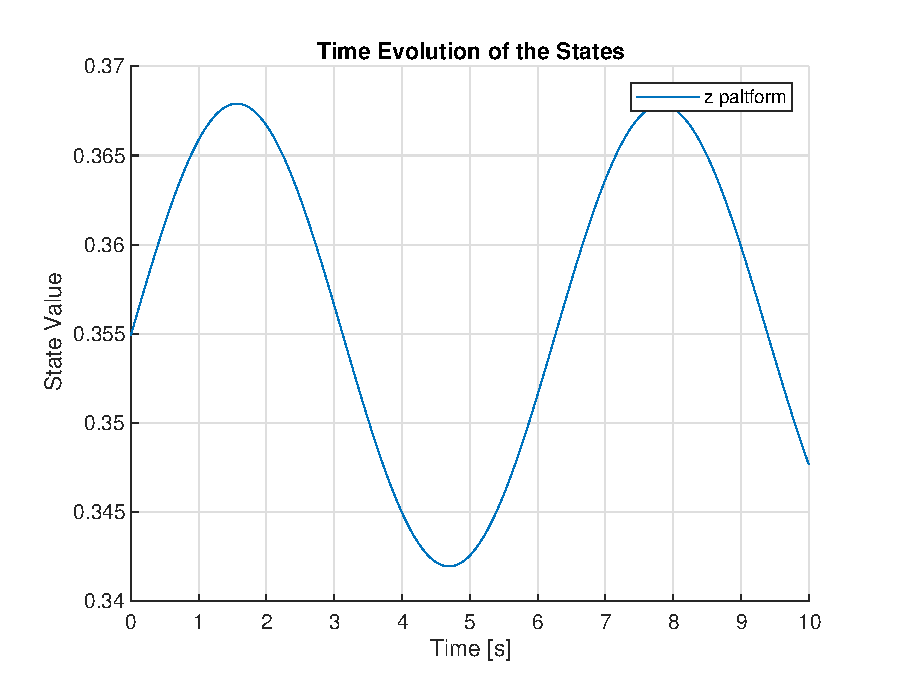
\includegraphics[width=\linewidth]{figure_6.eps} \\[0.5em]
	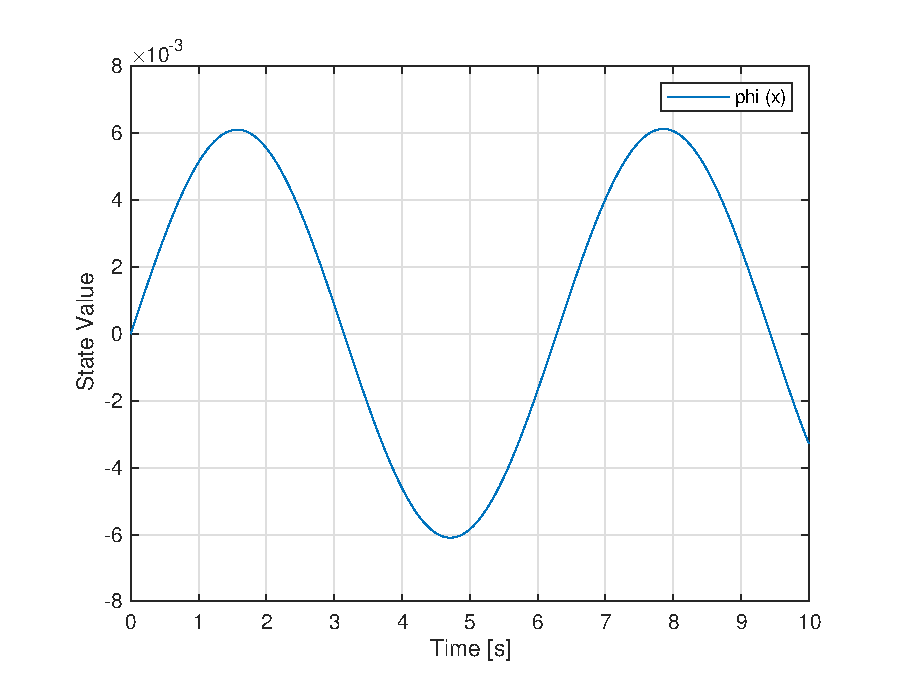
\includegraphics[width=\linewidth]{figure_7.eps} \\[0.5em]
	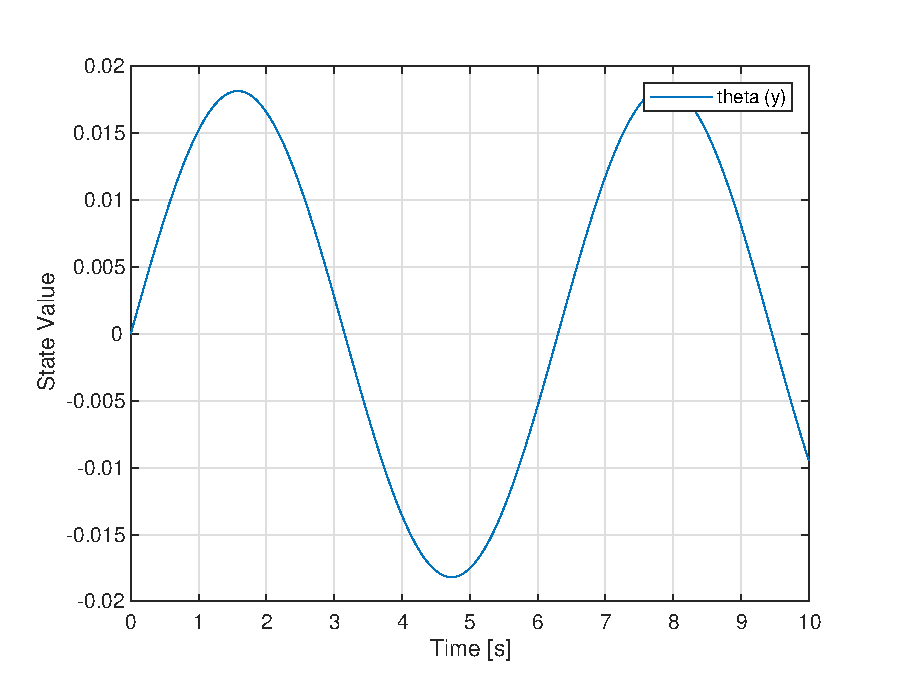
\includegraphics[width=\linewidth]{figure_8.eps}
\end{minipage}
\hfill
\begin{minipage}[t]{0.49\textwidth}
	\centering
	\textbf{Impulse} \\[0.3em] % ← title for column B
	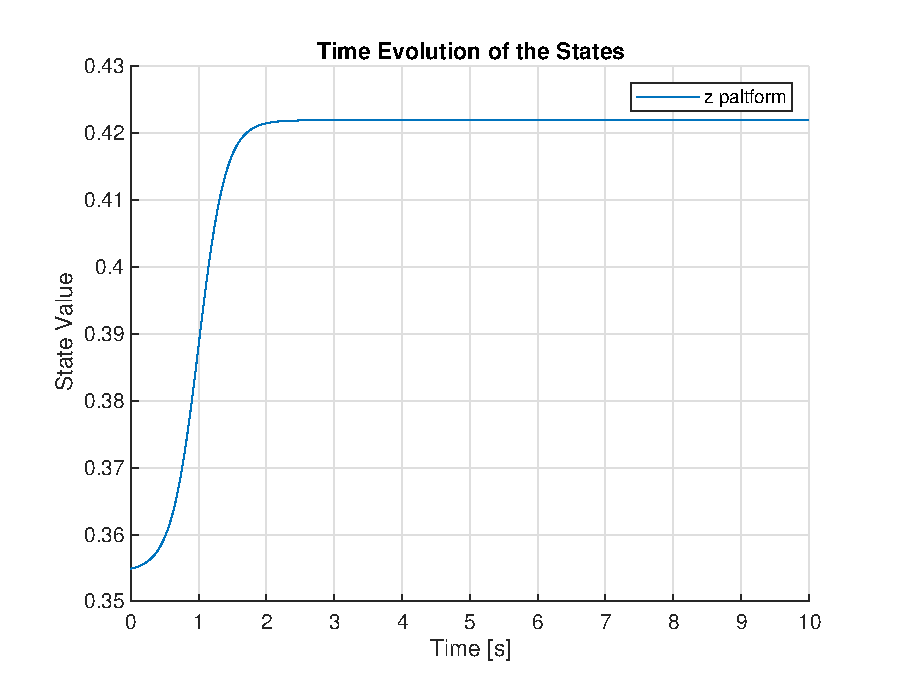
\includegraphics[width=\linewidth]{figure_9.eps} \\[0.5em]
	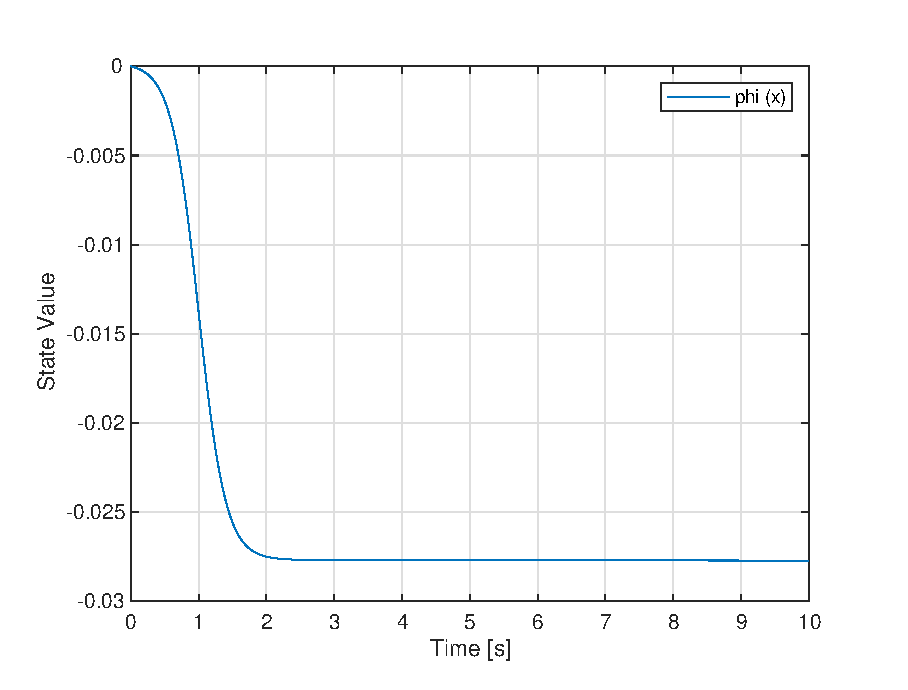
\includegraphics[width=\linewidth]{figure_10.eps} \\[0.5em]
	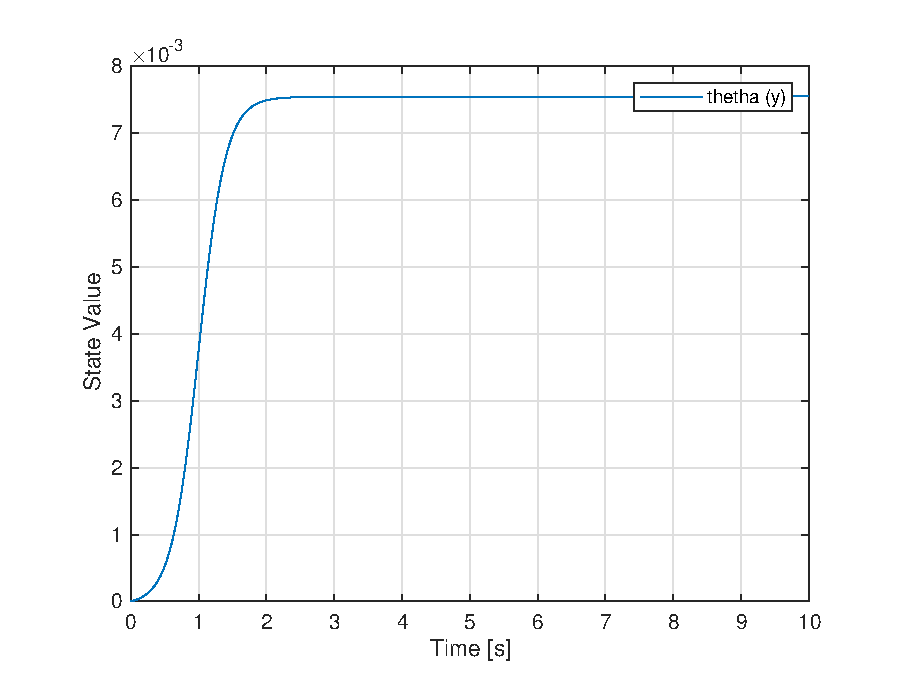
\includegraphics[width=\linewidth]{figure_11.eps}
\end{minipage}
\newpage
\matlabtitle{Simscape Model}

\begin{par}
\begin{flushleft}
To illustrate its dynamic response, the attached video shows the platform's behavior when three sinusoidal movements are applied to the actuators.
\end{flushleft}
\end{par}


\begin{par}
\begin{flushleft}
To validate the mathematical model, the same sinusoidal and impulse inputs were applied to the simscape model. The resulting platform movement was observed to be identical to the behavior predicted by the previously developed model, confirming its accuracy.
\end{flushleft}
\end{par}


\begin{figure}[H]
	\centering
	\begin{minipage}[b]{0.49\textwidth}
		\centering
		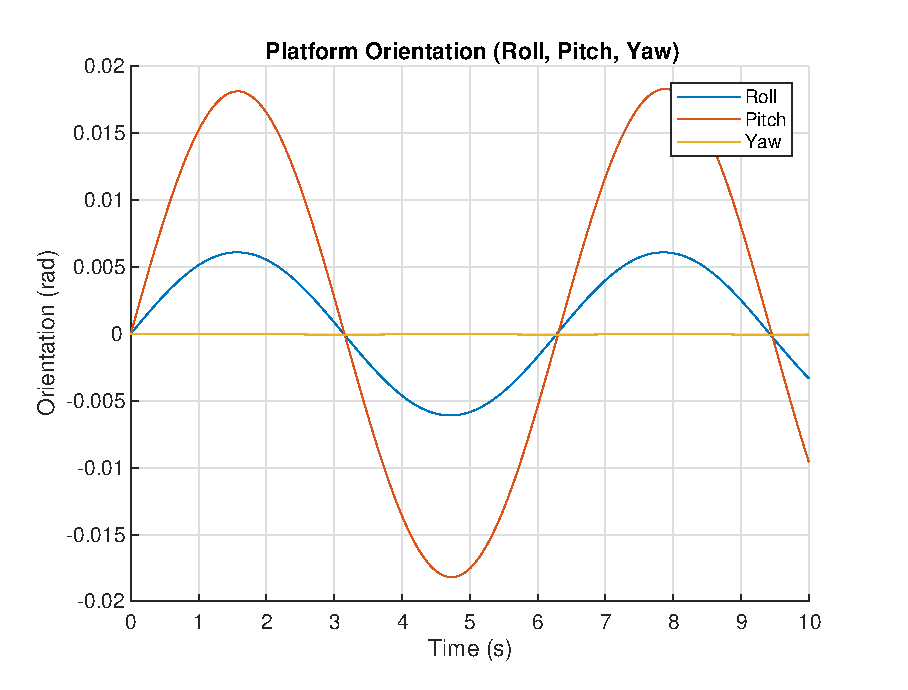
\includegraphics[width=\linewidth]{figure_12.eps}

	\end{minipage}
	\hfill
	\begin{minipage}[b]{0.49\textwidth}
		\centering
		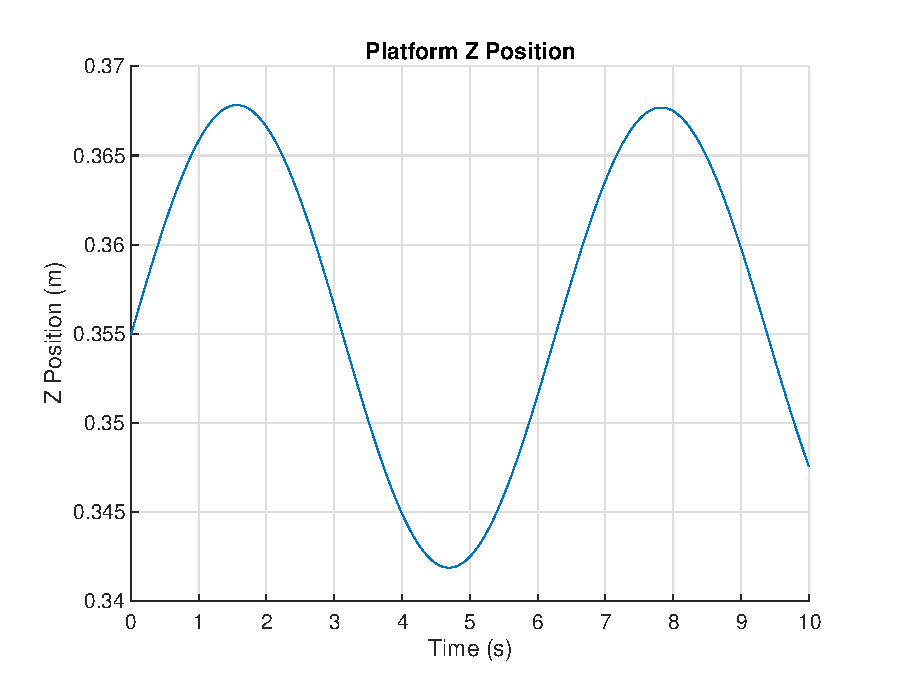
\includegraphics[width=\linewidth]{figure_13.eps}
	\end{minipage}
	
	\vspace{0.5cm} % space between rows
	
	\begin{minipage}[b]{0.49\textwidth}
		\centering
		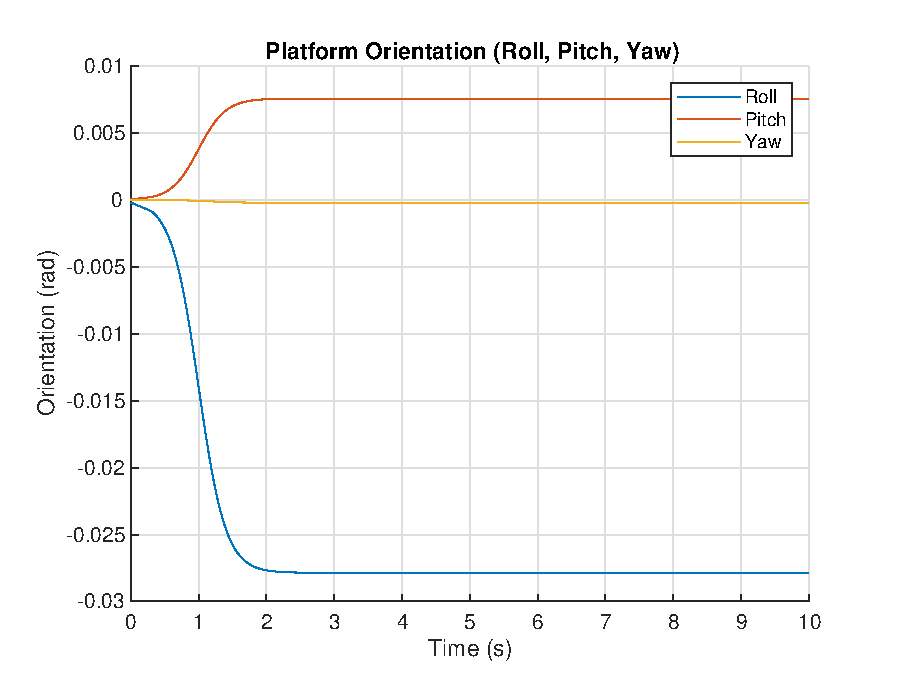
\includegraphics[width=\linewidth]{figure_14.eps}
	\end{minipage}
	\hfill
	\begin{minipage}[b]{0.49\textwidth}
		\centering
		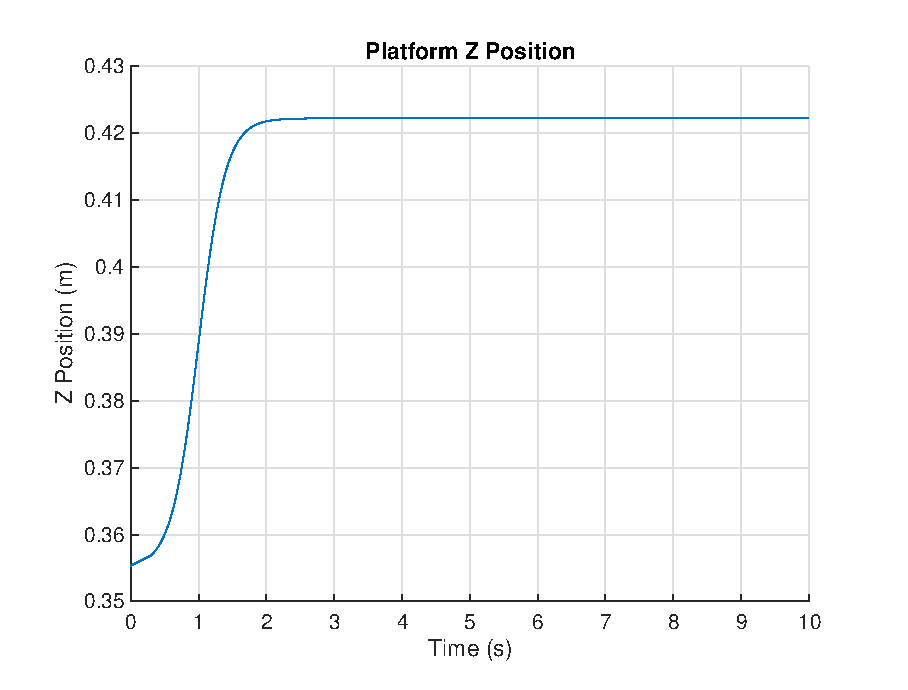
\includegraphics[width=\linewidth]{figure_15.eps}
	\end{minipage}
\end{figure}

\newpage

\begin{par}
	\begin{flushleft}
		The Simscape model was created following the same considerations as the mathematical model, in order to validate its results. As can be seen from the images, the architecture of the physical model mirrors the matlab one:
		\begin{figure}[H]
			\centering
			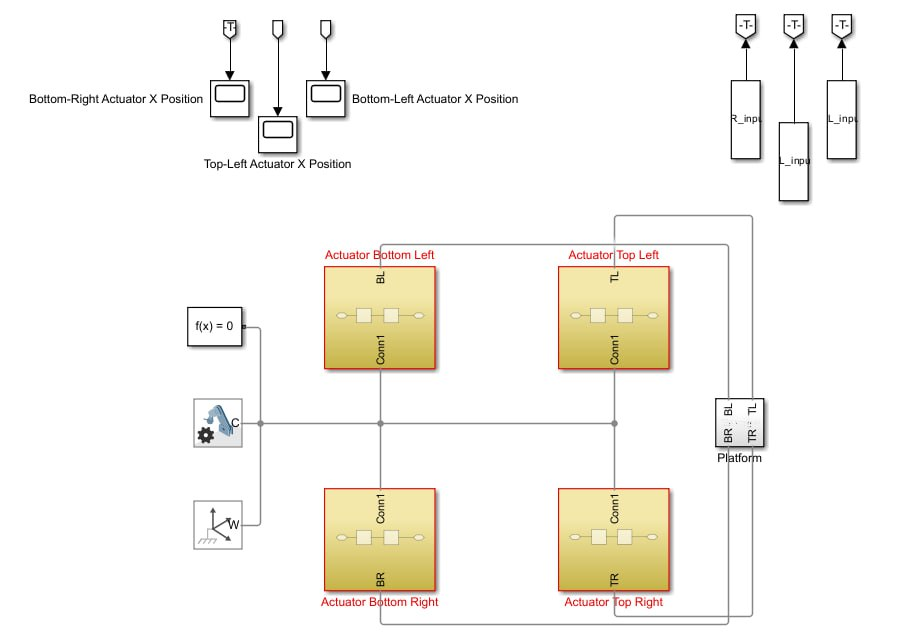
\includegraphics[width=0.6\linewidth]{sim_2}
			\caption{General scheme of the model}
			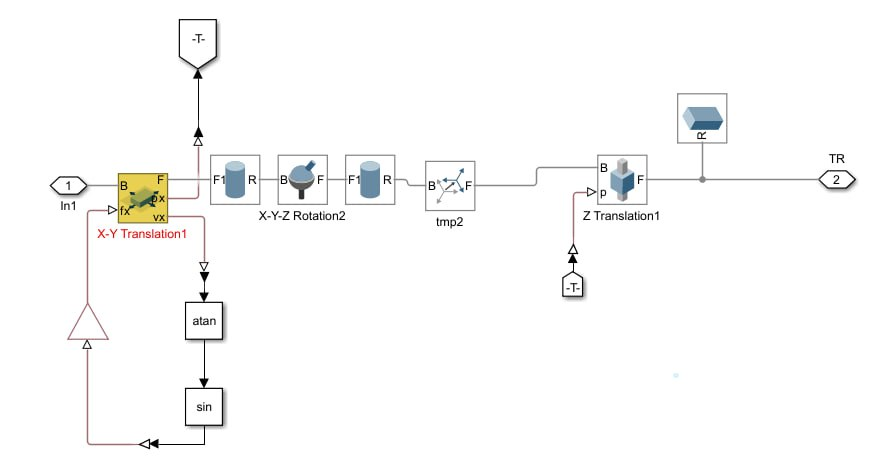
\includegraphics[width=0.6\linewidth]{sim_1}
			\caption{Non fixed actuator model}
		\end{figure}
		
		\begin{itemize}
			\item For each moving foot, a planar joint was inserted that allows its free movement along the $x$ and $y$ axes of the base plane.
			\item In succession, a revolute joint and a prismatic joint were applied to model the actuator.
			\item Unlike the mathematical model, a friction force was also applied to the foot, implemented via a feedback loop based on its velocity.
		\end{itemize}
		
		The fact that the results of the two models are identical  further confirms the validity of the key assumptions made during the analytical derivation, in particular:
		\begin{itemize}
			\item The small-angle approximation is correct.
			\item The assumption that the rotation of the actuators is the same as the platform's is valid for the system's kinematics.
		\end{itemize}
	\end{flushleft}
\end{par}


\newpage
\matlabtitle{Conclusion}

\begin{par}
\begin{flushleft}
Despite its utility, the developed model has inherent limitations that distinguish it from the behavior of a real system. These limitations stem from both the physical configuration of the platform and the assumptions made during the modeling phase.
\end{flushleft}
\end{par}

\begin{par}
\begin{flushleft}
\textbf{1. Degrees of Freedom (3-DOF vs. 6-DOF)}
\end{flushleft}
\end{par}

\begin{par}
\begin{flushleft}
The most significant limitation of the system lies in its 3 degrees of freedom (heave, pitch, roll), compared to the 6-DOF of a real vehicle. The absence of lateral (sway), longitudinal (surge), and vertical axis (yaw) rotation prevents the direct reproduction of fundamental driving sensations, such as:
\end{flushleft}
\end{par}

\begin{itemize}
\setlength{\itemsep}{-1ex}
   \item{\begin{flushleft} Sustained acceleration or braking (related to surge). \end{flushleft}}
   \item{\begin{flushleft} Lateral slip or centrifugal forces in a turn (related to sway). \end{flushleft}}
   \item{\begin{flushleft} Vehicle rotation or yaw (related to yaw). \end{flushleft}}
\end{itemize}

\begin{par}
\begin{flushleft}
\textbf{2. Physical Constraints and Motion Cueing Algorithms}
\end{flushleft}
\end{par}

\begin{par}
\begin{flushleft}
 The platform operates within defined physical limits, which prevent it from replicating the movements of a real vehicle on a 1:1 scale. Added to this are the intrinsic limits of the actuators, whose maximum velocity ($800 mm/s$) and acceleration ($0.8 g$) are specified in the datasheet.
\end{flushleft}
\end{par}

\begin{par}
\begin{flushleft}
These physical constraints necessitate the use of motion cueing algorithms. Such algorithms are tasked with "translating" the vehicle's dynamics and accelerations into platform movements that, while remaining within the limited workspace, manage to provide the driver with a plausible sense of motion. However, this introduces two compromises:
\end{flushleft}
\end{par}

\begin{itemize}
\setlength{\itemsep}{-1ex}
   \item{\begin{flushleft} High-Frequency Events: The platform's ability to reproduce road vibrations or rapid impacts is limited by the maximum acceleration of the actuators. \end{flushleft}}
   \item{\begin{flushleft} Command Saturation: If a simulated maneuver requires an acceleration exceeding 0.8 g, the control algorithm must "clip" or filter the command, delivering a movement that is compatible with the physical limits but loses realism for the driver. \end{flushleft}}
\end{itemize}

\begin{par}
\begin{flushleft}
\textbf{3. Modeling Assumptions}
\end{flushleft}
\end{par}

\begin{par}
\begin{flushleft}
The model is based on several key assumptions that, although justified to simplify the analysis, introduce discrepancies with real-world behavior:
\end{flushleft}
\end{par}

\begin{itemize}
\setlength{\itemsep}{-1ex}
   \item{\begin{flushleft} Small-Angle Approximation: Although verified a posteriori, this remains a simplification compared to the real, nonlinear kinematics, especially during large maneuvers. \end{flushleft}}
   \item{\begin{flushleft} Platform as a Rigid Body: This assumption ignores possible structural flexibilities or deformations of the platform, which could introduce secondary dynamics. \end{flushleft}}
   \item{\begin{flushleft} Friction Neglected: Is possible that the  friction (viscous in the actuators or sliding in the joints) plays a non-negligible role. The absence of friction in this model leads to an unrealistic estimation of energy consumption and long-term positioning accuracy. \end{flushleft}}
\end{itemize}

\begin{par}
\begin{flushleft}
Every assumption, however small, introduces a discrepancy between the model and reality. However, the choice of the level of approximation represents a fundamental engineering trade-off between model fidelity and its computational complexity. The definition of this balance is up to the modeler, in accordance with the specific goals and requirements of the project.
\end{flushleft}
\end{par}

\end{document}
